\chapter{Simulation results}

In this chapter we shall present a collection of the most interesting results obtained to validate the numerical performance of the discretization method described in the previously chapters. 

\section{Test cases}

We focus our tests over three kind of semiconductor devices: 

\begin{itemize}
\item {\bf p-n junction}
\item {\bf p-n junction in oxide}
\item {\bf MOSFET n-channel}
\end{itemize}

For everyone of these test cases we shall investigate the correctness of the FEMOS solution against the results obtained with SDEVICE.  
Furthermore we hang out some interesting comments about the performances of the solver and particular physical behaviours of the devices.

\subsection{p-n junction}
\label{sec: PN}

In this example we consider a simple p-n junction, also known as diode. In \figref{fig: diodo struttura} we present the partition used and the doping profile of this test case. The section of the parallelepiped is a $0.05 \times 0.05 [\mu m^2]$ square while the device is $0.1 [\mu m]$ long.  The number of verticises used is $4933$.  The doping concentration is obtained setting a constant profile of acceptor over all the domain ($N_A = 1.0\times 10^{17}$) overhelmed by a doping profile of acceptor ($N_D=1.0 \times 10^{18}$) bounded on one side of the device. As you can see we defined the two different areas of doping with an almost abrupt junction. 
Two contacts are defined, then on the first (A) is applyed a voltage of $0.3[V]$ while the opposite one (B) is grounded. In this situation the diode is direct polarized. The  relative electric permettivity of the silicon is $\epsilon_{SI} = 11.6 [F cm^{-1}]$ while the mobility model used is the thermal model \referenzaeq{eq: mobility thermal} with a constant temperature of $300 [K]$.

\begin{figure}[!t]
\centering
\subfloat[][\emph{Mesh}]
{\includegraphics[height=3.5cm]{Results/DIODE/AAA_structureandcontactFINITO.png}}
\hspace{1cm}
\subfloat[][\emph{Doping concentration}]
{\includegraphics[height=3.5cm]{Results/DIODE/AAADopingConcentrationFINITO.png}}
\label{fig: diodo struttura}
\end{figure}


In \ref{fig: diode potential}, \ref{fig: ndensity} and \ref{fig: pdensity} we validated FEMOS results against SDEVICE. As we aspected from theory the drop in potential is almost bounded around the junction, and as we use an asymmetric doping, it is major extended in the p-side. Notice that on the minority contact, which means A contact for electron solution and B contact for hole solution, the Dirichlet condition causes a big drop in concetration (from $1.0\times 10^{8}$ to $1.0 \times 10^3$ $[cm^{-3}]$). 

Now we are interested to analyze the computational performance. We know that the main difficulty is the initialization of the variables and obiouvsly the convergence time is strictly related to the kind of initial step we use. However predict in every situations the possibly shape of the solutions is hard, if not even impossible. For this reason a common and general approach is used: we split the domain in several regions accordingly to their doping concentration. Once obtained this partition we treat every of those semiconductor regions as they are in equilibrium with the nearest contact. This hypotesis allow us to compute over the entire domain the initial step for $\varphi$, $n$ and $p$ thanks to the relations \referenzaeq{eq: non eq n density mb} and \referenzaeq{eq: non eq p density mb}. 


\begin{figure}[!h]
\centering
\subfloat[][Total time Gummel Map. \label{fig: tempi computazionali 1}]
{\includegraphics[height=5cm]{Results/Caratteristiche/Diode/ComputationalTimeDifferentMeshes.eps}}
\subfloat[][Time NLP and DD, iteration GM. \label{fig: tempi computazionali 2}]
{\includegraphics[height=5cm]{Results/Caratteristiche/Diode/ConfrontoTempiNLPDDGMiterations.eps}}
\caption{Computational times for different bias.}
\end{figure}

Although some difficulties may occur, especially if we consider the device far away the equilibrium condition. We can state this effect looking at the figure \figref{fig: tempi computazionali 1}, where computational costs are shown against the polarization.
As expected if we spent more verticies for the discretization, the shape of the curve shift rigidly.
Although we notice that at $1.0[V]$ the computational time increases really quickly. For the simulated device this voltage level is almost the $built-in$ value. We are not surprised that first difficulties start from this voltage, indeed the solution becomes more different from the initial step used as you can see in \ref{fig: different biast initial step}.
A further proof of this problem could be found in \figref{fig: tempi computazionali 2}, where we show how this slowdown is related to the number of iterations of the Gummel Map and not to the properties of the linear problems solved. In fact while the number of iterations increases like the total time computation, the curves related to the computational time of NLP and DD solver equation remain unchanged.

\begin{figure}[!h]
\centering
\subfloat[][]
{\includegraphics[height=5cm]{DatiImmaginiTESI/Diode/PotentialZaxis01volt.eps}}
\subfloat[][]
{\includegraphics[height=5cm]{DatiImmaginiTESI/Diode/PotentialZaxis15volt.eps}}
\caption{Initial step for different bias.}
\label{fig: different biast initial step}
\end{figure}
 



%\begin{figure}[!h]
%\centering
%\includegraphics[scale=0.8]{Results/Caratteristiche/Diode/ConfrontoTempiNLPDDGMiterations.eps}
%\caption{Computational times and iterations.}
%\label{fig: times and iterations}
%\end{figure}




\clearpage 

\begin{figure}[!h]
\centering
\subfloat[][\emph{FEMOS}]
{\includegraphics[height=3.7cm]{Results/DIODE/FEMOS1817_potential03volt.png}}
\hspace{1cm}
\subfloat[][\emph{SDEVICE}]
{\includegraphics[height=3.7cm]{Results/DIODE/SDEVICE1817_potential03voltONLYDEVICE.png}}
\caption{Test case dide p-n 0.3[V] potential.}
\label{fig: diode potential}
\end{figure}

\vspace{1cm}

\begin{figure}[!h]
\centering
\subfloat[][\emph{FEMOS}]
{\includegraphics[height=3.7cm]{Results/DIODE/FEMOS1817_edensity03volt.png}}
\hspace{1cm}
\subfloat[][\emph{SDEVICE}]
{\includegraphics[height=3.7cm]{Results/DIODE/SDEVICE1817_edensity03voltONLYDEVICE.png}}
\caption{Test case dide p-n 0.3[V] electron density.}
\label{fig: ndensity}
\end{figure}

\vspace{1cm}

\begin{figure}[!h]
\centering
\subfloat[][\emph{FEMOS}]
{\includegraphics[height=3.7cm]{Results/DIODE/FEMOS1817_hdensity03volt.png}}
\hspace{1cm}
\subfloat[][\emph{SDEVICE}]
{\includegraphics[height=3.7cm]{Results/DIODE/SDEVICE1817_hdensity03voltONLYDEVICE.png}}
\caption{Test case dide p-n 0.3[V] hole density.}
\label{fig: pdensity}
\end{figure}


\clearpage


\subsection{p-n junction in oxide}
\label{sec: PNOX}

In this test case we surrounded the previous structure with a layer of oxide material ($\epsilon_{ox} = 3.7 [F cm^{-1}]$). This layer is about $0.025[\mu m]$ thick and notice that the contacts are defined only on the silicon region. We spent $6334$ verticies overall the domain. The structure and the doping are well defined in \figref{fig: structure diodeox}. The setting of the electrode is the same of the previously simulation. We still validate our solutions with the commercial software in \figref{fig: potential diodeox}, \figref{fig: edensity diodeox} and \figref{fig: hdensity diodeox}.  

\vspace{0.5cm}

\begin{figure}[!h]
\centering
\subfloat[][\emph{Mesh}]
{\includegraphics[height=4.5cm]{Results/DIODEOX/AAA_structureandcontact2.png}}
\hspace{1.5cm}
\subfloat[][\emph{Doping concentration}]
{\includegraphics[height=4.5cm]{Results/DIODEOX/AAA_Dopingconcentration2ONLYDEVICE.png}}
\caption{Test case p-n junction in oxide.}
\label{fig: structure diodeox}
\end{figure}

\vspace{0.5cm}

It's interesting notice that inside the oxide layer the potential seems to be more diffused than in the silicon. This phenomena becomes clear if we think about the relation \referenzaeq{eq: relazione pot electric} between electric field and potential.
 As we imposed $\nabla \varphi \cdot \vect{n}=0$ on the oxide boundary no field lines of the electric field could cross that boundary. The conseguence is that all the field lines could start and end only from the contact A or B.
Therefore the behaviour of the the electric field inside the device is due only to the displacement effect in the junction of the silicon, which imposes the electric response in the oxide material, see \figref{fig: electric field diode}. The conseguence is a lower electric field in the oxide, which implies a more diffused potential.


One of the most important issue that you have to keep in mind using a displacment approach on conservation law is that the pricinple of action reaction is not satisfied in a strong manner.
In this framework this statement means that given two element $K_i,K_j\in \mathcal{T}_h$ such that $K_i \bigcap K_j = f_i$ where $f_i \in \mathcal{F}_h$ and let be  $\vect{n}_{i}$ the outward normal vector of $\partial K_i$ and $\vect{n}_{j}$ the outward normal vector of $\partial K_j$,  we can't ensure that the following equations are verifyed

\begin{align}
\vect{D}|_{K_i}\cdot \vect{n}_{i} & = \vect{D}|_{K_j} \cdot \vect{n}_{j} \label{eq: conservazione vettore spostamento}\\
\vect{J}_n|_{K_i}\cdot \vect{n}_{i} & = \vect{J}_n|_{K_j}\cdot \vect{n}_{j} \\
\vect{J}_p|_{K_i}\cdot \vect{n}_{i} & = \vect{J}_p|_{K_j}\cdot \vect{n}_{j} 
\end{align}


If we consider \referenzaeq{eq: conservazione vettore spostamento} along the interface silicon-oxide and we fix the $x$ coordinate, we have

\begin{equation}
\epsilon_{ox}\vect{E}|_{K_i}\cdot \vect{n}_{i} = \epsilon_{Si}\vect{E}|_{K_j} \cdot \vect{n}_{j} \psp{5} \Rightarrow \psp{5}  [\vect{E}|_{K_i}]_y = \dfrac{\epsilon_{Si}}{\epsilon_{ox}}[\vect{E}|_{K_j}]_y
\end{equation}  

Accordingly with the parameters used during the simulations $\epsilon_{Si}/\epsilon_{ox}=3.22$, but as we expected by using the displacement approach we can't obtain this relation on the interface silicon-oxide. In \ref{fig: salto electric field} we present a plot along the Y axis, as you can see the ratio on the two interfaces are almost $3.9$. Furthermore every interfaces of the partition are affected by this problem, which means that inside an omogenous material the normal component of the electric field doesn't conserve. Even the presence of this drawback of the method, the solutions obtained well represent the physical behaviour of the devices, although it's important keep in mind this unavoidable criticality.

Finally we present some intersting plots which better validate our solutions with the commercial sofware. In these plots it's possible appreciate the big drop in concentration for the minority carriers at contacts and the boundary layers formed by the quasi fermi potentials.

\begin{figure}[!b]
\centering
\subfloat[][\emph{FEMOS}]
{\includegraphics[height=4.5cm]{Results/DIODEOX/FEMOS1817_electricfield03volt.png}}
\hspace{1.5cm}
\subfloat[][\emph{SDEVICE}]
{\includegraphics[height=4.5cm]{Results/DIODEOX/SDEVICE1817_electricfield03voltONLYDEVICE.png}}
\caption{Test case dide p-n in ox 0.3[V], electric field.}
\label{fig: electric field diode}
\end{figure}


\begin{figure}[!t]
\centering

\subfloat[][\emph{Electric field Y component.}]
{\includegraphics[height=4.7cm]{DatiImmaginiTESI/DiodeOx/ElectricFieldYaxis.eps}}
\subfloat[][\emph{Potential $V_A=0.3[V]$.}]
{\includegraphics[height=4.7cm]{DatiImmaginiTESI/DiodeOx/PotentialZaxis.eps}}

\subfloat[][\emph{Hole and electron densities.}]
{\includegraphics[height=4.7cm]{DatiImmaginiTESI/DiodeOx/DensityZaxis.eps}}
\subfloat[][\emph{Hole and electron quasi fermi potential}]
{\includegraphics[height=4.7cm]{DatiImmaginiTESI/DiodeOx/QFPotentialZaxis.eps}}
\end{figure}




\clearpage


\begin{figure}[!h]
\centering
\subfloat[][\emph{FEMOS}]
{\includegraphics[height=4.5cm]{Results/DIODEOX/FEMOS1817_potential03volt.png}}
\hspace{1cm}
\subfloat[][\emph{SDEVICE}]
{\includegraphics[height=4.5cm]{Results/DIODEOX/SDEVICE1817_potential03voltONLYDEVICE.png}}
\caption{Test case dide p-n in ox 0.3[V].}
\label{fig: potential diodeox}
\end{figure}

\vspace{0.5cm}

\begin{figure}[!h]
\centering
\subfloat[][\emph{FEMOS}]
{\includegraphics[height=4.5cm]{Results/DIODEOX/FEMOS1817_edensity03volt.png}}
\hspace{1cm}
\subfloat[][\emph{SDEVICE}]
{\includegraphics[height=4.5cm]{Results/DIODEOX/SDEVICE1817_edensity03voltONLYDEVICE.png}}
\caption{Test case dide p-n in ox 0.3[V].}
\label{fig: edensity diodeox}
\end{figure}

\vspace{0.5cm}

\begin{figure}[!h]
\centering
\subfloat[][\emph{FEMOS}]
{\includegraphics[height=4.5cm]{Results/DIODEOX/FEMOS1817_hdensity03volt.png}}
\hspace{1cm}
\subfloat[][\emph{SDEVICE}]
{\includegraphics[height=4.5cm]{Results/DIODEOX/SDEVICE1817_hdensity03voltONLYDEVICE.png}}
\caption{Test case dide p-n in ox 0.3[V].}
\label{fig: hdensity diodeox}
\end{figure}

\clearpage









\subsection{MOSFET n-channel}
\label{sec: MOS}

The functionality of a \textit{MOSFET} device is quite complex, therefore we give a summary of its basic operation. For a more detailed description see \textcolor{red}{referenza per mos}.
The metal-oxide-semiconductor field-effect transistor (MOSFET) is the building block of VLSI circuits in microprocessors and dynamic memories. Because the current in a MOSFET is transported predominantly by carriers of one polarity, the MOSFET is usually referred to as a unipolar or majority-carrier device.
In this test case we consider an \textit{n-channel MOSFET} or \textit{nMOSFET} which consists of a p-type silicon substrate into which two n-regions are formed. 
Its structure is well defined in \figref{fig: mos geometry}. It is a four-terminal device with the electrodes designated as gate (G), source (S), drain (D) and substrate or bulk (B). The gate electrode is usually made of metal or heavily doped polysilicon and is separated from the substrate by a thin silicon dioxide. The surface region under the gate  oxide between source and drain is called the \textit{channel} region.
We describe briefly the basic operation of a MOSFET device.
When there is no voltage applied to the gate there is no current flow between the source and drain, while if a sufficiently large positive voltage is applied to the gate, the silicon surface is inverted to n-type, which forms a conducting channel between the source and drain. In the latter case if we apply a voltage to the drain the electrons start to flow from source to drain and therefore a current in the opposite direction is generated. 
As we know already where the phenomena shall be more interesting we performed an oriented meshing which is high fitted along the channel region, at the contact and over the deplation region \figref{fig: mos geometry}. The n-regions are implanted accordingly with a gaussian profile.


\vspace{1cm}

\begin{figure}[!h]
\centering
\subfloat[][\emph{Mesh}]
{\includegraphics[height=4.2cm]{Results/MOS/AAA_MeshAndContact.png}}
\hspace{0.5cm}
\subfloat[][\emph{Doping concentration}]
{\includegraphics[height=4.2cm]{Results/MOS/AAA_DopingConcentrationONLYDEVICE.png}}
\caption{Geometry of the test case MOS n-channel.}
\label{fig: mos geometry}
\end{figure}




\begin{figure}[!h]
\centering
\subfloat[][\emph{$V_G=0.0[V]$, $V_D=0.1[V]$}]
{\includegraphics[scale=0.55]{DatiImmaginiTESI/Mos/BandDiagramMOS0volt.eps}}
\subfloat[][\emph{$V_G=2.0[V]$, $V_D=0.1[V]$}]
{\includegraphics[scale=0.55]{DatiImmaginiTESI/Mos/BandDiagramMOS2volt.eps}}
\caption{Energy band levels.}
\label{fig: energy levels MOS}
\end{figure}


We match our result in the operating phase of the MOSFET, therefore the setting of the electrode is $V_G=2.0[V]$, $V_D=0.1[V]$ and $V_S=V_B=0.0[V]$. The results are shown in \ref{fig: potential mos}, \figref{fig: ndensity mos} and \figref{fig: pdensity mos}. . The voltage applyed to the gate tends to decrease the band levels in the channel region: in this configuration the drain voltage causes the flow of the electron as the energy barrier doesn't exist anymore (see \figref{fig: energy levels MOS}).

Whereas the channel region belong to the p-region, with this polarization its nature is changed to an n-region. This means that a large concentration of electrons tends to form and the drain and the source terminals are put in contact. This phenomena is well described in \figref{fig: channel figures}.

Finally we propose in \figref{fig: electric field mos} a streamline plot of the electric field inside the device and the analogous graph performed with the SDEVICE solution.

\vspace{0.5cm}

\begin{figure}[!h]
\centering
\subfloat[][]
{\includegraphics[height=4.5cm]{DatiImmaginiTESI/Mos/DensityZaxis.eps}}
\hspace{1cm}
\subfloat[][]
{\includegraphics[height=4.5cm]{Results/PlotOverLine/Mos/Contour3DSpacechargeONLYDEVICE}}
\caption{Channel}
\label{fig: channel figures}
\end{figure}




\clearpage

\begin{figure}[!h]
\centering
\subfloat[][\emph{FEMOS}]
{\includegraphics[height=4.5cm]{Results/MOS/FEMOS181718_potential2voltONLYDEVICE.png}}
\hspace{0.8cm}
\subfloat[][\emph{SDEVICE}]
{\includegraphics[height=4.5cm]{Results/MOS/SDEVICE181718_potential2voltONLYDEVICE.png}}
\caption{Potential Vgate = 2.0 [V].}
\label{fig: potential mos}
\end{figure}

\vspace{0.5cm}

\begin{figure}[!h]
\centering
\subfloat[][\emph{FEMOS}]
{\includegraphics[height=4.5cm]{Results/MOS/FEMOS181718_ndensity2voltONLYDEVICE.png}}
\hspace{0.8cm}
\subfloat[][\emph{SDEVICE}]
{\includegraphics[height=4.5cm]{Results/MOS/SDEVICE181718_ndensity2voltONLYDEVICE.png}}
\caption{Electron density Vgate = 2.0 [V].}
\label{fig: ndensity mos}
\end{figure}

\vspace{0.5cm}

\begin{figure}[!h]
\centering
\subfloat[][\emph{FEMOS}]
{\includegraphics[height=4.5cm]{Results/MOS/FEMOS181718_pdensity2volt.png}}
\hspace{0.8cm}
\subfloat[][\emph{SDEVICE}]
{\includegraphics[height=4.5cm]{Results/MOS/SDEVICE181718_pdensity2voltONLYDEVICE.png}}
\caption{Electron density Vgate = 2.0 [V].}
\label{fig: pdensity mos}
\end{figure}


\begin{figure}[!t]
\centering
\subfloat[][\emph{FEMOS}]
{\includegraphics[height=4.5cm]{Results/MOS/FEMOS181718_ElectricField2voltONLYDEVICE.png}}
\hspace{1cm}
\subfloat[][\emph{SDEVICE}]
{\includegraphics[height=4.5cm]{Results/MOS/SDEVICE181718_ElectricField2voltONLYDEVICE.png}}
\caption{Electric field density Vgate = 2.0 [V].}
\label{fig: electric field mos}
\end{figure}

\subsubsection{Negative concentration}

In section \ref{sec: continuity equations} we admitted that the discretization scheme EAFE can't satisfy the discrete maximum principle in 3D simulations, therefore it's possible encounter negative concentration even if they are physical inconsistent. This situation often occurs when there are low densties of electrons or holes. In order to perform this event we produce the following test case on the MOSFET n-channel: all contacts are grounded then the drain is ramped to $0.5 [V]$. We are stressing the junction drain-bulk and as a consequence a large drop of the electron density occurs in the bulk region between the drain and the bulk. 

First simulations are performed with the partition previously presented (almost 3000 verticies). The solutions of the electron density computed with FEMOS and SDEVICE are shown in \figref{fig: negative carriers MOS}. As you can see the results are comparable, but near the drain-bulk junction the FEMOS solution presents some points with negative concentrations. However we obatin a good shape of the solution, but if we force beyond the polarization, the phenomenon will tend to spread over a larger area, untill it affects irremediably the computation.

The most practice technique to avoid this problem is the fitting of the mesh around the interested regions. Therefore we accomplished a second simulation with a new partition (with almost 13000 verticies), which is shown in \figref{fig: drain stress mos 13000}. As we expected the correct result is recovered and negative concentrations disappear from the solution. \textcolor{red}{possibile adattibilità di griglia?referenze?}.

It's interesting analyse how the fitting influences the satisfaction of the condition \referenzaeq{eq: extended criterion}. In \figref{fig: zikatanov mos} is well notable that in the drain-bulk junction side of the fitted mesh, the criterion is better fulfilled.


\begin{figure}[!h]
\centering
\subfloat[][\emph{FEMOS}]
{\includegraphics[height=4.5cm]{Results/Drainstress/NegativeCarrierOnlydevice.png}}
\hspace{1cm}
\subfloat[][\emph{SDEVICE}]
{\includegraphics[height=4.5cm]{Results/Drainstress/CarrierSDEonlydevice.png}}
\caption{Negative carriers in the electron density solution.}
\label{fig: negative carriers MOS}
\end{figure}

\begin{figure}[!h]
\centering
\subfloat[][\emph{Mesh 13000}]
{\includegraphics[height=4.5cm]{Results/Drainstress/MosMeshFitted.png}}
\hspace{1cm}
\subfloat[][\emph{FEMOS}]
{\includegraphics[height=4.5cm]{Results/Drainstress/NegativeCarrier13000onlydevice.png}}
\caption{Contribution of the impact ionization with the Van Over streaten model.}
\label{fig: drain stress mos 13000}
\end{figure}

\begin{figure}[!h]
\centering
\subfloat[][\emph{Coarse.}]
{\includegraphics[height=4.5cm]{Results/Drainstress/Zikatanov3000.png}}
\hspace{1cm}
\subfloat[][\emph{Fitted.}]
{\includegraphics[height=4.5cm]{Results/Drainstress/Zikatanov13000.png}}
\caption{Contribution of the impact ionization with the Van Over streaten model.}
\label{fig: zikatanov mos}
\end{figure}


\clearpage


\section{Current at contacts}

During the analysis of an electric device, one of the most useful information is the electrical response at terminals. In order to accomplish this target we have to compute the integral of the electron and hole current density over a generic electrode. A contact is defined by a surface and more precisely we can consider $\Gamma_{D,Si} = \bigcup_{c=1}^d \Gamma_c$ where $d$ is the number of terminals on the device and $\forall c=1,...,d$, $\Gamma_c$ is the $c$-th contact. The problem is $\forall c$ compute:

\begin{equation}
\mathcal{I}_c = \mathcal{I}_c^n + \mathcal{I}_c^p
\end{equation}

where $\mathcal{I}_c$ is the total current, $\mathcal{I}_c^n$ is the contribution of the electron current and $\mathcal{I}_c^p$ is the contribution of the hole current.
In general, given a contact $\Gamma_c$, fluxes of current density to be calculated assume the following form:

\begin{equation}
\label{eq: current flux}
\mathcal{I}_c^\nu = \int_{\Gamma_c}\vect{J}_\nu(\nu) \cdot \vect{n} \, d{\Gamma} \psp{10} \nu = \{n,p\}
\end{equation}

where as usual $\vect{n}$ is the unit outward normal of the domain boundary. It's well known that the evaluation of boundary integrals is a difficult task. Many difficulties in the numerical evalutaion of \referenzaeq{eq: current flux} arise from singularities in spatial derivatives of the approximate solution $n_h$ or $p_h$ near the contact edges, due to a change in the boundary condition type (e.g. from Dirichlet to Neumann) at the contact ends.

In the following we present an accurate method, known as \textit{residue method}, for the evaluation of boundary integrals in semiconductor device based on the work \cite{ContactCurrentRM}, we shall extend this technique to the 3D case and we confirm the optimal results matching them with SDEVICE. Moreover we remark that the method can be succesfully applied to a wide spread of applications, including contact charges, carrier quantum probability fluxes and heat fluxes.

The analysis made in \cite{ContactCurrentRM} are easily extendable to  our case if we consisder also the work made in \cite{GalerkMethConsHughes}. 



Consider the discretized electron continuity problem \referenzaeq{eq: weak formulation displacement} and let be $\eta$  the set of all vertices of the partition $\mathcal{T}_h$.  We can split the set of total nodes in contact node $\eta_g \in \Gamma_{D,Si}$ and the complementary part $\eta_n \in \Gamma_{N,Si}$. We define an \textit{auxiliary flux} $H_h$ on $\Gamma_{D,Si}$ as

\begin{equation}
H_h = \sum_{i\in\eta_g} H_{h,i} \psi_i 
\end{equation}


Now given the spaces:

\begin{align*}
\mathcal{V}_h = & span\{\psi_i\}_{i \in \eta_n} \\
\vect{V}_h = & span\{\psi_i\}_{i \in \eta_g}  \\
\mathcal{S}_h = & \{u \in \mathcal{V}_h \oplus \vect{V}_h: u|_{\Gamma_{D,Si}} = n_D \}
\end{align*}

it's possible write a modified form of Glakerin's method which reads as: 

find $n_h  \in \mathcal{S}_h$ and $H_h \in \vect{V}_h$ such that

\begin{equation}
\label{eq: modified galerkin}
(W_h,H_h)_{\Gamma_{D,Si}} = a(W_h,n_h)-F(W_h) \psp{10} \forall W_h \in \mathcal{V}_h \oplus \vect{V}_h
\end{equation}

where $a(\cdot,\cdot)$ is the bilinear form \referenzaeq{eq: weak formulation displacement} and $F(\cdot)$ the relative functional.
Equation \referenzaeq{eq: modified galerkin} splits into two subproblems:

\begin{align}
0  & = a(w_h,n_h)-F(w_h) \psp{10} \forall w_h \in \mathcal{V}_h \label{eq: usual problem}\\
(W_h,H_h)_{\Gamma_{D,Si}} & = a(W_h,n_h)-F(W_h) \psp{10} \forall W_h \in \vect{V}_h \label{eq: flux problem}
\end{align}

Problem \referenzaeq{eq: usual problem} it's identical to the unmodified case and we can manage it as we did untill now or adopt a different discretization scheme. Once obtained the solution $n_h$ problem \referenzaeq{eq: flux problem} is fully decoupled from \referenzaeq{eq: usual problem} and we can determines $H_h$ as follows

\begin{equation}
\label{eq: flux problem complete}
(H_h,\psi_i)_{\Gamma_{D,Si}} = a(\psi_i,n_h)-F(\psi_i) \psp{10} \forall i \in \eta_g 
\end{equation} 


In \cite{GalerkMethConsHughes} is demonstrated that $H_h$ defines the conserved total flux along $\Gamma_{D,Si}$ and accordingly with the boundary condition, the following equality is obtained

\begin{equation}
\label{eq: conservative flux}
\int_{\Gamma_{D,Si}} H_h \, d\Gamma = - \int_{\Omega_{Si}} qR \, d \Omega
\end{equation}


On the other hand if we apply the Divergence theorem on \referenzaeq{eq: LEC system} we can state 

\begin{equation}
\label{eq: lec divergence theor}
\int_{\Gamma_{D,Si}} \vect{J}_n \cdot \vect{n} \, d\Gamma = \int_{\Omega} - qR \, d\Omega
\end{equation}

Equation \referenzaeq{eq: conservative flux} and \referenzaeq{eq: lec divergence theor}  lead us to conclude that for all contacts we have

\begin{equation}
\label{eq: flux current formula}
\mathcal{I}_c^n = \int_{\Gamma_c} H_h \, d\Gamma
\end{equation}

In order to compute \referenzaeq{eq: flux current formula} let be $\eta_{c}$ the set of nodes of the contact $\Gamma_c$, the following equalities hold

\begin{equation}
\label{eq: equalities integrals}
\sum_{l \in \eta_c} \int_{\Gamma_c} H_h \psi_l \, d\Gamma 
=  \int_{\Gamma_c} H_h \sum_{l \in \eta_{c}} \psi_l \,d\Gamma 
= \int_{\Gamma_c} H_h \, d\Gamma
\end{equation}


Accordingly with  \referenzaeq{eq: equalities integrals} we can reinterpret $(H_h,\psi_i)_{\Gamma_{D,Si}}$ as the contribution to the flux at node $i$ and therefore the current at contact $c$ is given by summing over the verticies $\eta_{c}$ this quantity.

Therefore the residue method is:
given the system matrix $A$ of the Drif-Diffusion equation, the relative solution $n_h$ and the right hand side $\vect{b}$, $\forall c = 1,...,d$ the contribution to the total contact current is

\begin{equation}
\mathcal{I}_c^n = (An_h-\vect{b})\cdot \mathbb{I}_c
\end{equation} 

where

\begin{equation}
[\mathbb{I}_c]_i := \left\{ \begin{array}{ll}
0 & i \notin \eta_c \\
1 & i \in \eta_c
\end{array}  \right.
\end{equation} 

Obiouvsly the result is trivially extendable to the hole continuity equation. 

%Let be $A$ the system matrix of the continuity equation \referenzaeq{eq: matrice continuità} and $\vect{b}$ the relative right hand side before applying boundary conditions.  The linear problem looks as:
%
%\begin{equation}
%\label{eq: discretization before bc}
%\sum_{j\in\eta} A_{ij} \nu_j = b_i \psp{10} \forall i \in \eta
%\end{equation}
%
%
%Notice that the values of $\nu_j$ are known on the contacts and \referenzaeq{eq: discretization before bc} can be rewritten as follows:
%
%\begin{equation}
%\label{eq: discretization before bc 2}
%\begin{cases}
%
%\sum_{j\in\eta_n} A_{ij} \nu_j = b_i - \sum_{j\in\eta_g} A_{ij} \nu_j & \forall i \in \eta_n \\
%\\
%\sum_{j\in\eta_n} A_{ij} \nu_j = b_i - \sum_{j\in\eta_g} A_{ij} \nu_j & \forall i \in \eta_g \\
%
%\end{cases}
%\end{equation}
%
%The first set of equations is the usual linear system which we solve, while the second can be used for boundary flux estimation. 
% Now we define a new test function $v^h_i$ as:
%
%\begin{equation}
%\label{eq: new test function}
%v^h_i=\sum_{j\in\eta_{gi} }\psi_j
%\end{equation}
%
%where $\eta_{gi}$ is the set of nodes lying on $\Gamma_i$. Substituting \referenzaeq{eq: new test function} in \referenzaeq{eq: current flux} we can state that:
%
%\begin{multline}
%\mathcal{I}_i^\nu 
%= \int_{\Gamma_i}\vect{J}_\nu(\nu) \cdot \vect{n} \, d{\Gamma_i}
%= \sum_{j=1}^{n_d}\int_{\Gamma_j}\vect{J}_\nu(\nu) \cdot \vect{n} \,v_i^h \, d{\Gamma_j} \\
%=\sum_{i\in\eta_{gi}}\sum_{j=1}^{n_d}\int_{\Gamma_j}\vect{J}_\nu(\nu) \cdot \vect{n} \, \psi_i \, d{\Gamma_j} 
%= \sum_{i\in \eta_{gi}}\int_{\partial \Omega}\vect{J}_\nu(\nu) \cdot \vect{n} \, \psi_i \, d{\partial \Omega} \\
%= \sum_{i\in \eta_{gi}} \left[ \int_{\Omega}\nabla \cdot \vect{J}_\nu(\nu) \psi_i \, d{\Omega} + \int_{\Omega}\vect{J}_\nu(\nu) \cdot \nabla\psi_i \, d{\Omega} \right] \\
%= \sum_{m\in \eta_{gi}} \left[ \sum_{j\in\eta} A_{ij} \nu_j - b_i  \right] \\
%\end{multline}
%
%The current at contact $i$ is performed by summing the residuals of the matrix $A$.
%
%Per questo è detto metodo dei residui ...
%
%Nel seguito mostriamo alcuni risultati ...

\subsection{Results}

We shall apply the residue method over all the devices previously presented. Furthermore we treat specific condition of operation and different modelization of the mobility.

\subsubsection{p-n junction}

First of all we are intersted to reproduce the well known characteristic of the diode. Considering the device presented in section \ref{sec: PN} we grounded the B contact and then A contact is ramped from $-7.0[V]$ to $2.0[V]$. In  \figref{fig: caratteristica diode} we plot the magnitude in log scale of the contribution of the electron and hole current at contact A. In this case test we consider the constant mobility model. 
We notice that contact A is placed on the p-side of the device, where the holes are the majority carriers. The consequence is that the contribution to the current due to the impact ionization phenomenon is generated mostly by the hole flux. 
Breakdown voltage come up around $-7.0[V]$ and it's quite aligned with the one guess by SDEVICE.

\begin{figure}[!h]
\centering
\includegraphics[height=10cm]{Results/Caratteristiche/Diode/CaratteristicaDiode.eps}
\caption{Diode characteristic.}
\label{fig: caratteristica diode}
\end{figure}

\vspace{2cm}
Mettere un'altra immagine del diodo?



\clearpage



\subsubsection{p-n junction in oxide}

We obtained correct results also for the diode surrounded by the oxide. For this test case we analyzed the influence of the Masetti mobility model to the current. In order to appreciate significative changes, the device operates only in direct polarization between $0.0[V]$ and $1.5[V]$.
In \figref{fig: diode ox const} are shown the electron and hole current at contact A with the constant mobility model, while in \figref{fig: diode ox masetti} we switched on the Masetti model.The effect due to the dopant concentration is clearer in \figref{fig: diode ox masetti focus}, where a focus on the  operation region of the diode is made (above $0.8[V]$). As you can see the total current with Masetti mobility is lower and still aligned with the SDEVICE result.


\begin{figure}[!h]
\centering
\subfloat[][\label{fig: diode ox const}]
{\includegraphics[height = 4.5cm]{Results/Caratteristiche/DiodeOx/CurrentDiodeOxide.eps}}
\subfloat[][\label{fig: diode ox masetti}]
{\includegraphics[height = 4.5cm]{Results/Caratteristiche/DiodeOx/CurrentDiodeOxideMasetti.eps}}

\subfloat[][\label{fig: diode ox masetti focus}]
{\includegraphics[height = 4.5cm]{Results/Caratteristiche/DiodeOx/CurrentDiodeOxideConstantVsMasetti.eps}}

\caption{Direct polarization constant mobility.}
\end{figure}



%\begin{figure}[!h]
%\centering
%\caption{Direct polarization Masetti mobility.}
%\end{figure}
%
%\begin{figure}[!h]
%\centering
%
%\caption{Masetti mobility effect Vs. constant mobility effect.}
%\end{figure}



\clearpage

\subsubsection{MOSFET n-channel}

For the MOSFET n-channel we treat the follow sets of polarization:
\begin{itemize}
\item[1.] $I_D-V_G$ {\bf characteristic at low drain bias},  $V_S=V_B=0.0[V]$, $V_D=0.1[V]$, the gate contact is ramped from $-0.5[V]$ (MOS off) to $2.0[V]$ (MOS on);
\item[2.] $I_D-V_D$ {\bf characteristic MOSFET off}, $V_S=V_B=V_G=0.0[V]$ the drain contact is ramped from $0.0[V]$ to $1.0[V]$, in this case the MOS is off and we are stressing the drain-bulk junction;
\item[3.] $I_D-V_D$ {\bf characteristic MOSFET on}, $V_S=V_B=V_G=2.0[V]$, the drain contact is ramped from $0.0[V]$ to $0.2[V]$;
\end{itemize}

For the test case 1. we are interested to demonstrate the accuracy of all mobility models implemented. The current in a MOSFET is transported predominantly by carriers of one polarity, e.g. in a n-channel device by electrons, therefore the total current corresponds to the electron current contribution. 

\begin{figure}[!h]
\subfloat[][\label{fig: current drain mos direct}]
{\includegraphics[height=5cm]{Results/Caratteristiche/Mos/CurrentIDVG.eps}}
\subfloat[][\label{fig: current drain mos direct focus}]
{\includegraphics[height=5cm]{Results/Caratteristiche/Mos/CurrentIDVGfocus.eps}}
\end{figure}


\clearpage

Test case 2. was already presented in the previous section in order to treat problems of negative concentrations. Here we focus on the effect of the impact ionization phenomenon and the bulk current computation. A large amount of generation is produced around the drain junction while the polarization increases. In \figref{fig: II MOS} it's shown the contribution due to the Van Overstraeten - de Man model computed at $V_D = 0.5 [V]$ with FEMOS and SDEVICE. 

Under this condition no channel is formed beneath the oxide layer, therefore there isn't a preferential path which electrons may follow. As a consequence carriers can move from both source and bulk contact. In \figref{fig: tutte le correnti mos stress} this phenomenon is well predicted by FEMOS, indeed while the drain voltage increased the bulk current raise consistently.


\begin{figure}[!h]
\centering
\subfloat[][\emph{FEMOS}]
{\includegraphics[height=5cm]{Results/Drainstress/IIFEMOSonlydevice.png}}
\hspace{1cm}
\subfloat[][\emph{SDEVICE}]
{\includegraphics[height=5cm]{Results/Drainstress/IISDEonlydevice.png}}
\caption{Contribution of the impact ionization with the Van Overstraeten - de Man model.}
\label{fig: II MOS}
\end{figure}

\begin{figure}[!h]
\centering
\includegraphics[height=5cm]{Results/Caratteristiche/Mos/Inverse/MOScaratteristicaDrainstress.eps}
\caption{$I_D$, $I_B$ and $I_S$ against $V_D$.}
\label{fig: tutte le correnti mos stress}
\end{figure}




Test case 3.

Grafici non belli. Necessario? Esiste qualche set partiolare che fa notare comportamenti interessanti?